\documentclass[10pt]{standalone}
\usepackage{amsmath}
\usepackage{pgf,tikz}
\usepackage{mathrsfs}
\usetikzlibrary{arrows}
\pagestyle{empty}
\begin{document}
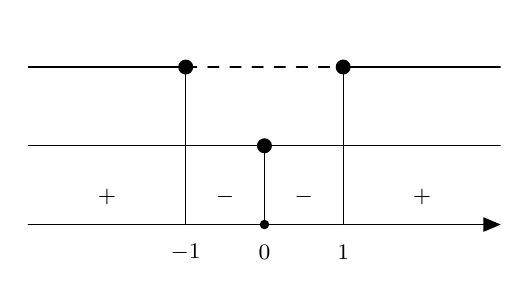
\begin{tikzpicture}[line cap=round,line join=round,>=triangle 45,x=1.0cm,y=1.0cm]
%\draw [color=black,, xstep=1.0cm,ystep=1.0cm] (-3.,-0.5) grid (3.,2.5);
\draw[->,color=black] (-3.,0.) -- (3.,0.);
%\foreach \x in {-3.,-2.,-1.,1.,2.}
%\draw[shift={(\x,0)},color=black] (0pt,2pt) -- (0pt,-2pt) node[below] {\footnotesize $\x$};
%\draw[->,color=black] (0.,-0.5) -- (0.,2.5);
%\foreach \y in {,1.,2.}
%\draw[shift={(0,\y)},color=black] (2pt,0pt) -- (-2pt,0pt) node[left] {\footnotesize $\y$};
\draw[color=black] (0pt,-10pt) node {\footnotesize $0$};
\draw[color=black] (1,-10pt) node {\footnotesize $1$};
\draw[color=black] (-1,-10pt) node {\footnotesize $-1$};
\draw[color=black] (-2,10pt) node {\footnotesize $+$};
\draw[color=black] (2,10pt) node {\footnotesize $+$};
\draw[color=black] (-0.5,10pt) node {\footnotesize $-$};
\draw[color=black] (0.5,10pt) node {\footnotesize $-$};
\clip(-3.,-0.5) rectangle (3.,2.5);
\draw (-1.,2.)-- (-1.,0.);
\draw (0.,1.)-- (0.,0.);
\draw (1.,2.)-- (1.,0.);
\draw (3.,1.)-- (-3.,1.);
\draw (-3.,2.)-- (-1.,2.);
\draw (1.,2.)-- (3.,2.);
\draw [dash pattern=on 4pt off 4pt] (-1.,2.)-- (1.,2.);
\begin{scriptsize}
\draw [fill=black] (0.,1.) circle (2.5pt);
\draw [fill=black] (-1,2) circle (2.5pt);
\draw [fill=black] (1,2) circle (2.5pt);
%\draw[color=black] (0.1287970441329163,1.3672006473974139) node {$C$};
\draw [fill=black] (0.,0.) circle (1.5pt);
%\draw[color=black] (0.05131790928999042,1.8708150238764323) node {$l$};
\end{scriptsize}
\end{tikzpicture}
\end{document}